\documentclass[oneside, final, 14pt]{extreport}
\usepackage[utf8]{inputenc}
\usepackage[russian]{babel}
\usepackage{vmargin}
\setpapersize{A4}
\setmarginsrb{2cm}{1cm}{1cm}{1cm}{0pt}{0mm}{0pt}{13mm}
\usepackage{indentfirst}
\usepackage{amsmath}
\usepackage{graphicx}
\usepackage{wrapfig}
\sloppy

\begin{document}
  
\setcounter{chapter}{2}
\chapter{Аналогово-цифровое и цифроаналоговое преобразование звука}
\section{Общие замечания}

Звук представляется в звуковой аппаратуре либо в виде непрерывного электрического сигнала, либо в закодированном цифровом виде. Аппаратура, в которой рабочим сигналом является непрерывный электрический сигнал, описывающий
звуковые колебания, называется {\itshape аналоговой аудиоаппаратурой} (например, бытовой магнитофон, аудиоусилитель, динамик, осциллограф и т.д.), а сам сигнал~--- аналоговым аудиосигналом.

В аналоговой звуковой аппаратуре информация о звуковой волне представляется в виде непрерывного электрического сигнала, моделирующего форму (вид) звуковой волны и ее параметры в функции времени на основе законов Ома и Кирхгофа
для электрической цепи. Устройством для преобразования звуковых колебаний в электрический (аналоговый) сигнал является микрофон, а аналогового сигнала звуковой частоты в звуковые колебания~--- акустический динамик (электродинамический громкоговоритель). Принцип действия микрофона и динамика основан на взаимодействии переменного тока, протекающего в электрической цепи катушки индуктивности, с магнитным полем постоянного магнита.

В динамике классической конструкции подвижная катушка индуктивности, жестко скрепленная с диафрагмой динамика, подключается к источнику электрического сигнала звуковой частоты (например, к аудиоусилителю). В результате
взаимодействия электрического тока, протекающего по катушке, с магнитным полем постоянного магнита катушка приходит в движение (колебания с частотой напряжения источника) в продольном направлении (т.е. по оси катушки), что, в свою
очередь, приводит к аналогичным колебаниям прикрепленной к катушке диафрагмы, которая и излучает звук (т.е. создает звуковую волну) с частотой колебаний напряжения на катушке.

В электродинамическом микрофоне упругая мембрана из тонкого металла, жестко соединенная с катушкой индуктивности, под действием переменного давления звуковой волны перемещается (колеблется) в магнитном поле с частотой звуковой
волны. С такой же частотой колеблется (перемещается вдоль оси мембраны) катушка индуктивности в магнитном поле постоянного магнита, в результате чего в ней индуцируется переменная Э.Д.С. (электродвижущая сила) с частотой колебания мембраны. Если электрическую цепь катушки подключить, например, к катушке записывающей головки магнитофона, то в образованной электрической цепи под действием Э.Д.С. будет протекать ток с частотой звуковой волны (звука), с помощью которого реализуется запись исходного звукового сигнала на магнитную ленту. Так происходит преобразование звуковых колебаний в аналоговый аудиосигнал.

Цифровая аппаратура оперирует дискретными, цифровыми сигналами. {\itshape Цифровой аудиосигнал}~--- это лишь форма (способ) записи аналогового сигнала, т.е. это аналоговый аудиосигнал, представленный некоторым образом в виде дискретных численных значений.

Преобразование аналогового звукового сигнала в цифровой вид называется {\itshape аналогово-цифровым преобразованием} или {\itshape оцифровкой}, а устройство, предназначенное для осуществления такого преобразования, называют {\itshape аналогово-цифровым преобразователем}, сокращенно~--- {\itshape АЦП} (Analog-to-Digital Converter~--- АDС). Процесс аналогово-цифрового преобразования с помощью АЦП заключается в осуществлении замеров текущих величин амплитуды аналогового сигнала с некоторым временным шагом и последующей записи полученных значений амплитуды в некоторой численной форме.

Наиболее общим примером цифрового устройства (т.е. электронного устройства, в котором рабочим сигналом является дискретный сигнал) является компьютер. В компьютере взаимодействие всех составляющих компьютер блоков происходит путем обмена и обработки одного или одновременно нескольких двоичных сигналов.

\section{Дискретизация и квантование}
\subsection{Дискретизация во времени}
Начальным этапом аналогово-цифрового преобразования сигнала является процесс дискретизации (осуществление выборки) сигнала во времени.

Этот этап преобразования мы называем "начальным" лишь условно, поскольку на самом деле процесс временной дискретизации и процесс квантования сигнала по уровню протекают одновременно пошагово в аналогово-цифровом преобразователе (АЦП).

\textit{Дискретизация во времени}~--- это процесс регистрации мгновенных значений амплитуды преобразуемого аналогового сигнала (измеряемой в вольтах) через определенные промежутки времени, т.е. с определенным временным шагом, называемым \textit{шагом дискретизации} (рис. \ref{pic-digital-01}). 

Номер шага дискретизации (в дальнейшем мы будем обозначать его $n$) условимся нумеровать от нуля, т.е. 0, 1, 2,...

\begin{figure}[h]
\centering
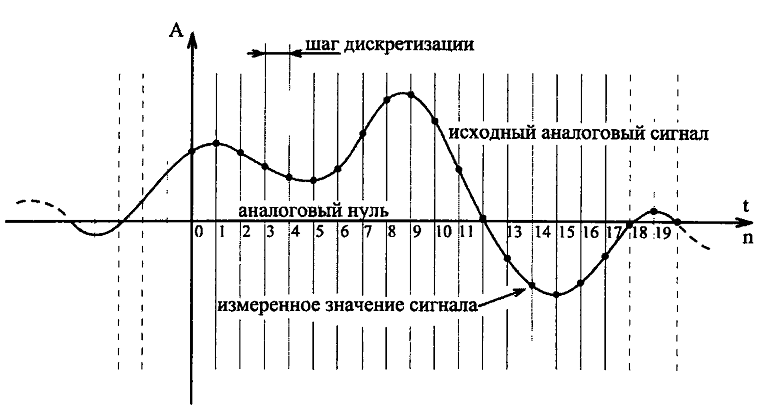
\includegraphics[width=0.75\textwidth]{pic-digital-01}
\caption{Иллюстрация процесса дискретизации исходного аналогового сигнала во времени}
\label{pic-digital-01}
\end{figure}

Количество осуществляемых в одну секунду замеров амплитуды сигнала называют \textit{частотой дискретизации} или \textit{частотой выборки}, или частотой сэмплирования (от англ. "<sampling">~--- "<выборка">, "<замер">). 

Как и всякая другая частота, частота дискретизации измеряется в герцах (Гц). Заметим здесь, что ось времени $t$ на рис. \ref{pic-digital-01} прочерчена в том месте, где проходит так называемый \textit{аналоговый нуль сигнала}~--- условная линия равновесия ("<тишины">) аналогового сигнала, т.е. линия условного нулевого значения амплитуды
аналогового сигнала, относительно которой совершаются колебания электрического тока, моделирующего колебания звуковой волны (звука).

В электрической цепи аналогового аудиоустройства протекает переменный ток, моделирующий звуковые колебания (звуковую волну). В отсутствии звуковых колебаний на аналоговую цепь подается постоянный потенциал некоторой величины (постоянное напряжение +11 В). Этот потенциал является аналоговым нулем. Звуковые колебания моделируются в аналоговом тракте колебаниями напряжения относительно аналогового нуля.

Очевидно, что чем меньше шаг дискретизации, тем выше частота дискретизации, т.е. тем чаще происходит регистрация значений амплитуды сигнала, тем более точное представление об аналоговом сигнале мы получаем. Эти рассуждения
подтверждаются \textit{теоремой Котельникова}. 

\emph{Согласно этой теореме, аналоговый сигнал с ограниченным спектром может быть точно описан дискретной последовательностью значений его амплитуды, если эти значения следуют с частотой, как минимум вдвое превышающей наивысшую частоту спектра.} 

Иначе говоря, аналоговый сигнал, в котором частота наивысшей составляющей спектра равна $F_m$, может быть точно описан последовательностью дискретных значений амплитуды, если для частоты дискретизации сигнала $F_d$ выполняется условие $F_d\geq2F_m$. 

На практике условие теоремы Котельникова означает следующее: для того, чтобы оцифрованный сигнал содержал информацию обо всем диапазоне слышимых человеком частот ($0 - 20$ кГц) исходного аналогового сигнала, частота дискретизации при оцифровке должна составлять не менее 40 кГц, т.е. 40000 замеров амплитуды в одну секунду. Отсюда нетрудно рассчитать минимальный временной шаг дискретизации, равный 0,000025 с = 25 мкс. Теорема Котельникова является фундаментальной и лежит в основе теории и практики цифровой обработки сигналов.

Казалось бы, что для завершения процесса оцифровки теперь остается лишь записать измеренные мгновенные значения амплитуды аналогового сигнала в численной форме; полученная последовательность чисел (по одному результату замера амплитуды сигнала на каждый шаг) и образует цифровую форму исходного аналогового сигнала~--- так называемый импульсный сигнал. Однако здесь и обнаруживается основная трудность оцифровки. Суть проблемы заключается в следующем.

С одной стороны, необходимо сохранить точность значений замеров амплитуды сигнала, т.е. сохранить как можно большее количество знаков после запятой.

С другой стороны, сделать это нужно в как можно более компактной форме с тем, чтобы в результате оцифрованные данные имели приемлемый объем. При этом компактность записи не должна повредить точности значения каждого отдельного замера амплитуды, так как в противном случае записанная последовательность чисел уже не сможет обеспечить необходимой точности описания исходного аудио-
сигнала, что в конечном итоге может отрицательно сказаться на качестве воспроизведения полученного цифрового сигнала.

Заметим попутно, что \emph{при оцифровке звуковых сигналов вполне достаточным условием является точная передача слышимого диапазона частот преобразуемого сигнала.}

Остальными частотами можно пренебречь, поскольку слушатель так или иначе не способен ощущать частоты выше 20-22 кГц. По этой причине значение частоты дискретизации цифрового аудиосигнала в пределах 40-44 кГц, в соответствии с теоремой Котельникова, вполне удовлетворяет требованиям качественной
передачи звучания. Дальнейшее повышение частоты дискретизации нецелесообразно, поскольку оно почти не способно повлиять на качество звучания, при этом оно может привести к нежелательному увеличению объемов данных. Вообще говоря, соображения целесообразности являются ключевыми во всем, что касается
цифровой аппаратуры и практической обработки сигналов, в том числе оцифровки сигналов. По большому счету именно соображения целесообразности, одновременно со стремлением достижения лучших результатов по комплексу параметров, лежат в основе всех цифровых технологий.

\subsection{Линейное (однородное) квантование}
Линейное (однородное) квантование звукового сигнала является одним из способов преобразования аналогового звукового сигнала в описывающую его последовательность чисел. В процессе линейного квантования непрерывный аналоговый звуковой сигнал представляется на каждом шаге дискретизации в виде прямоугольных импульсов текущей амплитуды. Поэтому аналоговая кривая в процессе линейного квантования приобретает ступенчатую форму и представляется непрерывной последовательностью прямоугольных импульсов различной величины, вписанных в аналоговую кривую.

Рассмотрим процесс линейного квантования подробнее и попутно приведем новые термины и понятия.

Допустим, что на запись одного измеренного значения амплитуды сигнала мы отводим строго $N$ бит. Одной $2^N$-битной записью можно представить любое десятичное число в диапазоне от $0$ до $2^{N-1}$, а значит, с помощью $N$ бит можно представить (описать) $2^N$ возможных различных значений амплитуды
сигнала.

Предположим теперь, что значения оцифровываемого аналогового сигнала колеблются в максимальных пределах от $-1$ до $+1$ некоторых условных единиц
(у.е.) относительно упомянутого нами аналогового нуля. Назовем этот диапазон значений аналогового сигнала \textit{динамическим диапазоном аналогового сигнала}. Таким образом, динамический диапазон аналогового сигнала составляет 2 у.е. 

Заметим, что измеряемые значения сигнала могут быть дробными (например, 0,126 у.е. или 0,997375 у.е.). Произведем разбиение амплитудной шкалы в пределах от $-1$ до $+1$ у.е. на $2^N-1$ равных интервалов (рис. \ref{pic-digital-02}), в результате чего на шкале получим $2^N$ горизонтальных отметок (линий). Каждую полученную
линию назовем \textit{квантом} (\textit{уровнем квантования}). 

Расстояние между двумя ближайшими уровнями квантования называется \textit{шагом квантования}, мы будем обозначать его $\Delta$. В рассматриваемом случае, когда динамический диапазон сигнала составляет 2 у.е., шаг квантования 
\[\Delta=2/{2^{N-1}}\text{~у.е.}\]~

\begin{figure}[h]
\centering
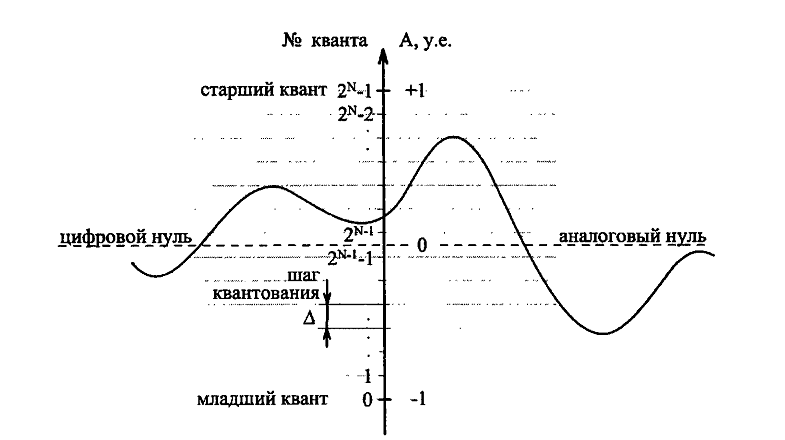
\includegraphics[width=0.75\textwidth]{pic-digital-02}
\caption{Разделение амплитудной шкалы на уровни квантования}
\label{pic-digital-02}
\end{figure}

Разделение амплитудной шкалы на равные промежутки называется \textit{линейным} или \textit{однородным}. Самый нижний уровень амплитуды, соответствующий минимальной расчетной величине входного сигнала ($-1$ у.е.), назовем младшим квантом, а самый верхний уровень, соответствующий максимальной расчетной величине ($+1$ у.е.),~--- старшим квантом. Кванты пронумеруем от $0$ до $2^N-1$. Таким образом, для записи номера некоторого кванта в двоичной форме нам понадобится $N$ бит (или $N/8$ байт) и не более. Линию, проходящую через отметку на оси ординат, расположенную ровно на половине расстояния между старшим и младшим квантами,
называют цифровым нулем (на рис. \ref{pic-digital-02} цифровой нуль расположен ровно между квантами с номерами $2^{N-1}-1$ и $2^{N-1}$. В идеальном случае значения цифрового нуля квантователя и аналогового нуля входного сигнала совпадают.

При записи каждого отдельного значения измеренной амплитуды преобразуемого аналогового сигнала это значение \textit{округляют} до ближайшего уровня (кванта). Этот процесс называется \textit{квантованием} исходного аналогового сигнала по амплитуде. Другими словами, \textit{квантование по амплитуде}~--- это процесс замены реальных (измеренных) значений амплитуды сигнала приближенными значениями с определенной точностью. 

Устройство, осуществляющее такое преобразование, называют квантователем. В случае линейного разбиения амплитудной шкалы на уровни квантование называют линейным (однородным), а квантователь, соответственно,~--- линейным квантователем. Разницу между величинами входного сигнала, соответствующими младшему и старшему квантам, называют динамическим диапазоном квантователя. 

На рис. \ref{pic-digital-03} представлена иллюстрация метода однородного квантования для общего случая. На рисунке продемонстрирован идеальный случай, когда цифровой нуль квантователя совпадает с аналоговым нулем сигнала.

\begin{figure}[h]
\centering
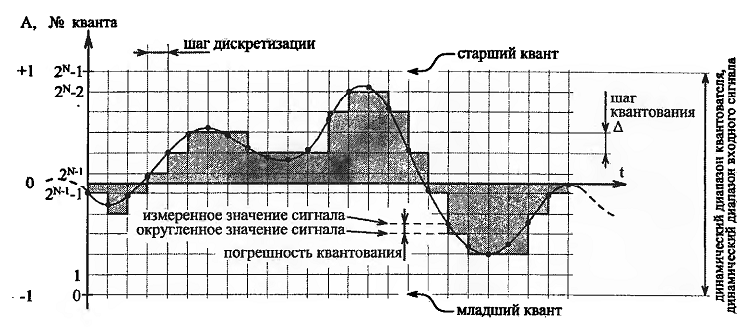
\includegraphics[width=0.75\textwidth]{pic-digital-03}
\caption{Разделение амплитудной шкалы на уровни квантования}
\label{pic-digital-03}
\end{figure}

Как видно из рис. \ref{pic-digital-03}, результатом дискретизации и квантования, т.е. результатом оцифровки аналогового сигнала, стал ступенчатый сигнал, составленный из прямоугольных импульсов, каждый из которых имеет ширину, равную величине шага дискретизации, и высоту, равную округленному (квантованному) значению амплитуды сигнала. Таким образом, можно сказать, что \textit{полученная последовательность квантованных значений амплитуды входного аналогового сигнала является цифровым описанием исходного сигнала, т.е. цифровым аудиосигналом}.

В качестве наглядного примера рассмотрим квантование аналогового сигнала с помощью трехбитного квантователя (т.е. для записи каждого квантованного значения сигнала отводятся $N=3$ бит). Таким образом, в распоряжении квантователя находятся $2^3=8$ квантов, т.е. 8 уровней квантования амплитуды входного аналогового сигнала, при этом шаг квантования $\Delta$ составляет $2/7$ у.е. (рис. \ref{pic-digital-04}).

\begin{figure}[h]
\centering
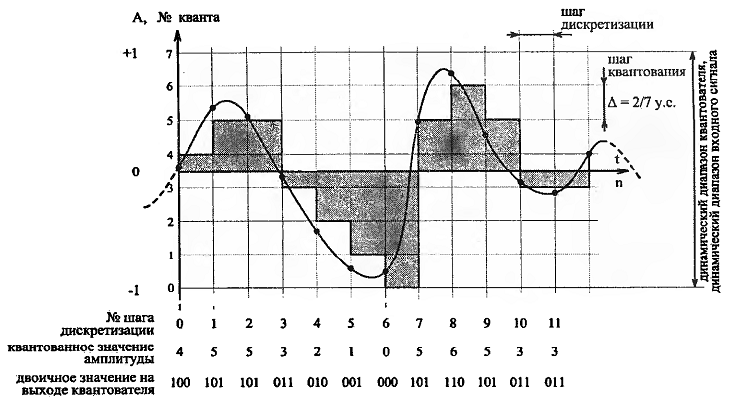
\includegraphics[width=0.75\textwidth]{pic-digital-04}
\caption{Пример квантования сигнала при $N=3$}
\label{pic-digital-04}
\end{figure}

На рисунке можно видеть разницу между измеренными значениями амплитуды сигнала и квантованными (округленными) значениями, форму ступенчатого сигнала, а также двоичные значения сигнала на выходе квантователя. 

Чтобы сохранить полученный цифровой сигнал, например, в памяти компьютера, достаточно сохранить последовательность чисел, считанную на выходе квантователя, т.е. квантованные значения амплитуды последовательно для каждого шага преобразования (шага дискретизации). В дальнейшем, зная величину шага дискретизации, на основе записанной последовательности чисел можно воссоздать ступенчатую форму исходного аналогового сигнала.

На рис. \ref{pic-digital-04} последовательность дискретных значений (т.е. номеров квантов), составляющая результирующий цифровой сигнал, выглядит как
\[4, 5, 5, 3, 2, 1, 0, 5, 6, 5, 3, 3\].

Она же в двоичной форме (теоретический вид) выглядит как
\[100, 101, 101, 11, 10, 1, 0, 101, 110, 101, 11, 11\].

В двоичной форме на выходе трехбитного квантователя получаем
\[100~101~101~011~010~001~000~101~110~101~011~011\]
(отсутствие запятых между числами указывает на то, что на практике эта последовательность представляет собой непрерывный трехразрядный бит-поток.)

Вернемся к вопросам квантования. Очевидно, что точность округления значений амплитуды зависит от выбранного количества уровней квантования $2^N$, которое, в свою очередь, зависит от количества $N$ бит, отведенных для записи значений амплитуд. Чем больше уровней квантования и чем ближе они друг к другу (т.е. чем меньше $\Delta$), тем на меньшую величину приходится округлять измеренные значения амплитуды в процессе квантования, и, таким образом, тем меньше получаемая \textit{погрешность квантования}. Число $N$ называют \textit{разрядностью квантования}, подразумевая при этом количество разрядов в двоичной записи одного квантованного значения амплитуды на выходе квантователя, а "<снятые"> с выхода квантователя округленные значения сигнала~--- \textit{отсчетами} или \textit{сэмплами}.

Эффективность квантования зависит от правильности выбора квантователя.

Если, например, динамический диапазон преобразуемого в цифровую форму аналогового сигнала будет превышать динамический диапазон квантователя, то на вход последнего могут попадать значения сигнала, превышающие максимально допустимые для квантователя, что приводит к "<зашкаливанию"> сигнала на входе квантователя. В этом случае квантователь "<обрезает"> сигнал на уровне, соответствующем его динамическому диапазону. Явление обрезывания сигнала называется \textit{клипированием или клиппингом} (от англ. "<clipping">~--- "<обрезывание">). 

Клиппинг, по сути, является результатом перегрузки сигнала на входе квантователя и приводит к возникновению в цифровом сигнале неприятных аудиопомех. 

На рис. \ref{pic-digital-05} представлен наглядный пример возникновения клиппинга.

\begin{figure}[h]
\centering
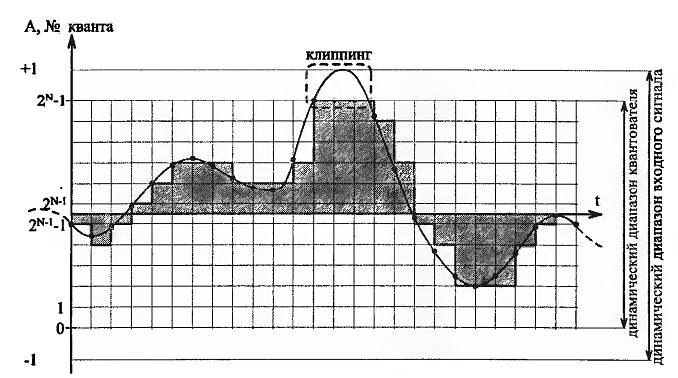
\includegraphics[width=0.75\textwidth]{pic-digital-05}
\caption{Пример возникновения клиппинга}
\label{pic-digital-05}
\end{figure}

Дополнительные проблемы в процессе оцифровки сигнала может вызвать несовпадение уровней аналогового и цифрового нулей, а точнее~--- смещение оси аналогового сигнала относительно цифрового нуля. Это несовпадение проявляется в случае неверного сопряжения аналоговой схемы со входом цифрового блока и самим АЦП. Расстояние между аналоговым и цифровым нулями называется \textit{сдвигом постоянной составляющей} или DC-офсетом (от англ. "direct current offset"~--- смещение постоянного тока). 

Описанный способ оцифровки сигнала, осуществляемой с помощью АЦП, а именно~--- дискретизация сигнала во времени в совокупности с методом линейного (однородного) квантования, называется \textit{импульсно-кодовой модуляцией}, \textit{ИКМ} (англ. Pulse Code Modulation - РСМ).

\begin{figure}[h]
\centering
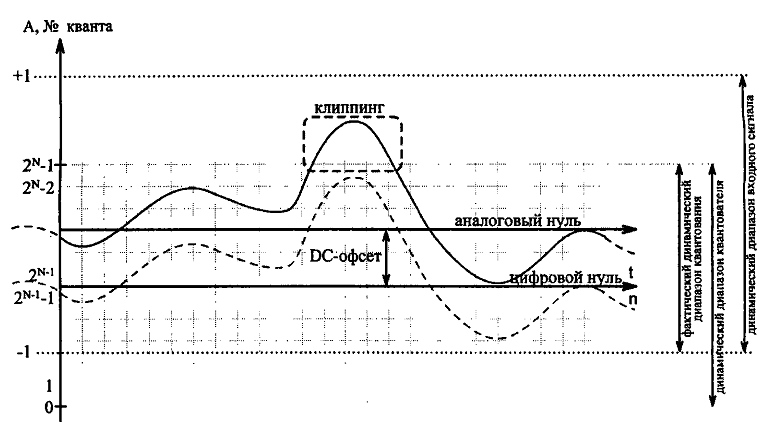
\includegraphics[width=0.75\textwidth]{pic-digital-06}
\caption{Пример наличия ненулевого DC-офсета}
\label{pic-digital-06}
\end{figure}

Стандартный аудио компакт-диск, применяемый с начала 80-х годов XX столетия, хранит информацию в формате ИКМ с частотой дискретизации 44,1 кГц и разрядностью квантования 16 бит (таким образом, один отсчет представляет значение амплитуды исходного аналогового сигнала числом от 0 до 65 535).

СD-DА (Compact Disc Digital Audio)~--- стандарт записи данных на оптических аудио компакт дисках. Стандарт устанавливает следующие параметры кодирования: двух- или одноканальная запись (т.е. стерео или моно) в формате ИКМ с частотой дискретизации 44,1 кГц и разрядностью квантования 16 бит. Одна секунда аудио в таком формате занимает 176 400 байт (2 канала $\times$ 44 100 отсчетов в секунду $\times$ 2 байт на отсчет) или 1 411 200 бит. Говорят, что битрейт (от англ. "<bit rate">~--- "<скорость бита">, "<скорость потока информации">) данных в формате СD-DА составляет 1 411 200 бит/с. Выходит, что один час аудио в этом формате занимает объем около 600 Мбайт (60 мин $\times$ 60 с $\times$ 2 канала $\times$ 44 100 отсчетов в секунду $\times$ 2 байт на отсчет = 605 Мбайт).

\section{Цифроаналоговое преобразование}
Чтобы яснее понять, почему точность округления при квантовании и частота дискретизации являются столь критичными параметрами оцифровки, рассмотрим процесс обратного преобразования цифрового сигнала в аналоговую форму. Но сначала сделаем небольшое отступление и ответим на два вопроса, которые уже как бы "<зависли в воздухе">: "<Зачем нужно выполнять обратное преобразование с таким трудом оцифрованного исходного аналогового сигнала?"> и "<Зачем вообще нужно кодировать звуковой сигнал?">.

Все дело в том, что цифровой и аналоговый аудиосигналы~--- это две формы представления оригинального звукового сигнала, придуманные человеком для того, чтобы сделать возможным эффективное хранение, обработку, анализ и воспроизведение звуковой информации. 

Закодированная в аналоговой или цифровой форме звуковая волна является промежуточной стадией в записи и воспроизведении
звука. Понятно, что набором цифр или аналоговой моделью звуковой волны не вызовешь колебания воздушной среды. Однако эти вспомогательные формы представления звука позволяют оперировать его параметрами и производить над ним необходимые действия. Из приведенного небольшого отступления следует, что для того, чтобы "<прослушать"> цифровой сигнал, нужно восстановить (декодировать) его аналоговый вид, т.е. представить цифровой звуковой сигнал в виде электрической модели, а именно~--- в виде непрерывных колебаний напряжения и тока в
электрической цепи, что, в свою очередь, будет аналогом механических колебаний диффузора и частиц воздушной среды.

Процесс восстановления аналогового сигнала из цифровой формы называется \textit{цифроаналоговым преобразованием}. Устройство, осуществляющее это преобразование, называется \textit{цифроаналоговым преобразователем}, \textit{ЦАП} (Digital to Analog Converter~--- DAC). Цифро-аналоговое преобразование представляет собой процесс, обратный процессу дискретизации: аналоговый сигнал "<реконструируют"> из импульсного сигнала путем интерполяции, беря определенное количество отсчетов (сэмплов) в единицу времени.

Как мы говорили выше, согласно теореме Котельникова, восстановление аналогового сигнала из цифровой формы может быть достаточно точным лишь в том случае, если использованная при оцифровке частота дискретизации $F_d$ как минимум в $2$ раза превышает частоту $F_m$ наивысшей спектральной составляющей исходного аналогового звукового сигнала, т.е. должно выполняться условие $F_d\geq2F_m$, отсюда
$F_m\leq F_d/2$. Если при оцифровке это условие выполнено не было, то точное восстановление полезной (прослушиваемой) части спектра аналогового сигнала оказывается невозможным.

Причина невозможности точного восстановления сигнала в случае невыполнения указанного условия заключается в следующем. Дело в том, что в результате дискретизации в частотном спектре цифрового (импульсного) сигнала появляется дополнительный спектр высших гармоник, располагающийся вокруг гармоник частоты дискретизации (т.е. вокруг спектральных составляющих с частотами $\nu F_d$ для $\nu=1, 2, 3, ...$) в диапазоне $D$, ширина которого равна удвоенной ширине $М$ спектра исходного аналогового сигнала. Эти высшие гармоники ("<паразитные"> спектральные компоненты) являются составляющими так называемых зеркальных отражений спектра исходного аналогового сигнала (рис. \ref{pic-digital-07}, а). 

Иными словами, в спектре импульсного сигнала вокруг частот $F_d, 2F_d, 3F_d,...$, появляются по две копии спектра исходного сигнала, одна из которых является зеркальным отражением другой. Этот эффект называется \textit{алиазингом} (от англ. "<alias">~--- "<псевдоним">).

Если $F_m$ превышает половину частоты дискретизации  (т.е. если $F_m>F_d/2$), то в результате дискретизации дополнительные паразитные компоненты (из состава зеркальных отражений) попадают в область $М$ исходного аналогового сигнала (см. рис. \ref{pic-digital-07}, б). В этом случае восстановить исходный сигнал без искажений из цифровой формы уже не удается.

\begin{figure}[h]
\centering
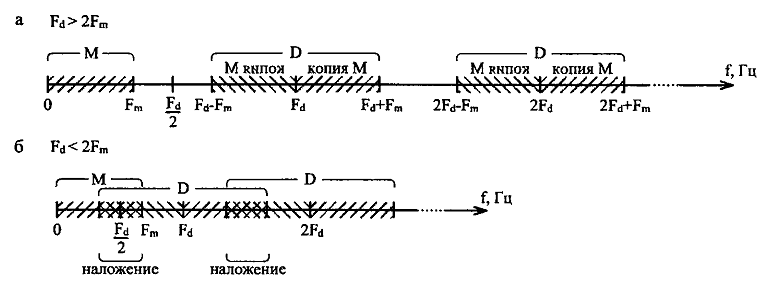
\includegraphics[width=0.75\textwidth]{pic-digital-07}
\caption{Диаграмма состава спектра импульсного сигнала}
\label{pic-digital-07}
\end{figure}

Процесс цифроаналогового преобразования на практике проходит фактически в два этапа:
\begin{itemize}
\item генерирование ступенчатого аналогового сигнала на основе известной информации об отсчетах цифрового сигнала, взятой, например, из памяти компьютера (ЦАП получает на входе последовательность отсчетов, т.е. цифровых значений сигнала, и выводит на выходе аналоговые импульсы соответствующей величины);
\item сглаживание импульсного аналогового сигнала с помощью аналогового фильтра нижних частот (ФНЧ) с частотой среза, равной половине частоты дискретизации.
\end{itemize}

ФНЧ на втором этапе используется с тем, чтобы отсечь от спектра ступенчатого аналогового сигнала указанные выше зеркальные отражения спектра и тем самым сгладить ступенчатую форму волны. На практике ввиду неидеальности ФНЧ частота дискретизации $F_d$ на этапе аналоговоцифрового преобразования выбирается несколько больше $2F_m$ т.е. "<с запасом">. 

\begin{figure}[h]
\centering
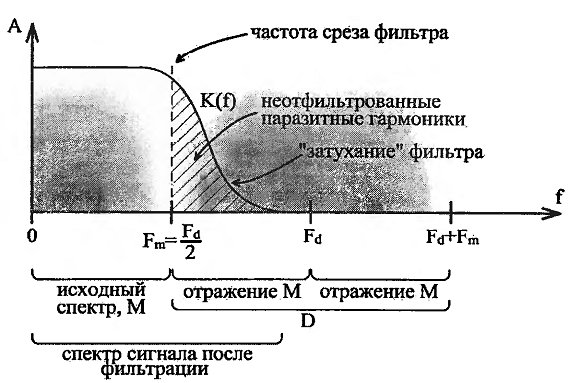
\includegraphics[width=0.75\textwidth]{pic-digital-08}
\caption{Иллюстрация необходимости применения ФНЧ при цифроаналоговом преобразовании}
\label{pic-digital-08}
\end{figure}

\section{Шум квантования}
\textit{Шумом квантования} называют аудиосигнал, составляющий разницу между аналоговым импульсным сигналом, восстановленным из цифрового сигнала на выходе ЦАП, и исходным аналоговым аудиосигналом (до оцифровки). 

Обозначим исходный аналоговый сигнал $A(t)$, а импульсный аналоговый сигнал, восстановленный из цифрового,~--- $D(t)$. Тогда шум квантования~--- это сигнал $N(t)=D(t)-А(t)$, отсюда $D(t)=A(t)+N(t)$. Фактически $N(t)$~--- это сигнал, каждый отсчет которого равен ошибке при округлении текущего значения амплитуды сигнала $A(t)$ до ближайшего уровня квантования (кванта) на соответствующем шаге процесса оцифровки сигнала $A(t)$. Другими словами, шум квантования~--- это те искажения, которые добавляются к исходному аналоговому сигналу в процессе его оцифровки.

Отсюда можно дать следующее определение цифровому (импульсному) звуковому сигналу $D(t)$: это исходный аналоговый сигнал $A(t)$ с подмешанным к нему шумом квантования $N(t)$. На рис. \ref{pic-digital-09} показана наглядная иллюстрация процесса образования шума квантования.

\begin{figure}[h]
\centering
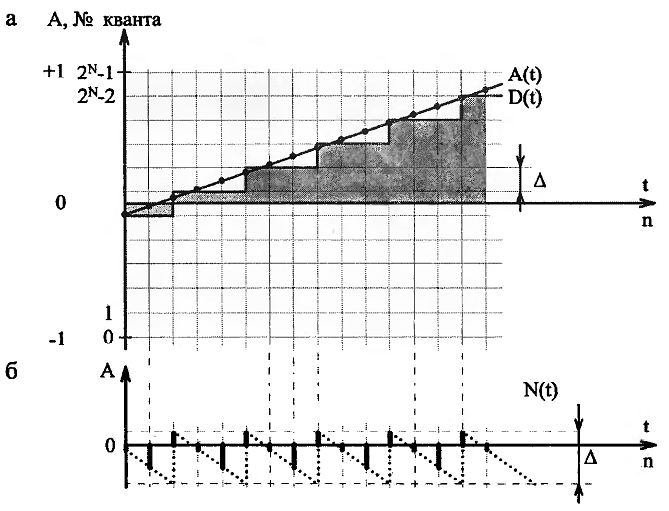
\includegraphics[width=0.75\textwidth]{pic-digital-09}
\caption{Иллюстрация образования шума квантования}
\label{pic-digital-09}
\end{figure}

На верхнем графике показаны аналоговый сигнал $А(t)$ в виде наклонной линии и образующийся в процессе его оцифровки импульсный сигнал $D(t)$. На нижнем графике приведена кривая $N(t)$ в виде пунктирной линии, огибающей ошибки, полученные в результате округления измеренных значений амплитуды сигнала $А(t)$ до ближайших уровней квантования (сплошные вертикальные жирные линии на каждом шаге дискретизации) в процессе его оцифровки, т.е. график шума квантования.

В целом, величина шума квантования, т.е. величина погрешности квантования на каждом шаге дискретизации, колеблется в пределах величины $\Delta/2$. Иными словами, разброс значений шума квантования не превышает $\Delta/2$. Поэтому, чем выше разрядность квантования (чем больше число квантов), тем ниже уровень шума квантования, поскольку с увеличением разрядности квантования шаг квантования
$\Delta$ уменьшается. В предельном случае, если ошибки квантования на каждом шаге дискретизации будут достигать их максимально возможного значения, общий (наибольший) уровень шума квантования, для данной разрядности квантования $N$ можно определить по известной зависимости:

\[S_i=20 \log(1/k)\text{~дБ,}\]
где $k=2^N$. 

Например, для 8-и разрядного преобразования $k=256, S_i=-48$~дБ.

\begin{table}[ht]
  \caption{Уровень шума квантовая}
  \begin{center}
  \begin{tabular}{|l|c|c|}
  \hline Разрядность, бит & $k$ & Уровень шума квантования, дБ\\
  \hline 1 & 2 & -6 \\  
  \hline 8 & 256 & -48 \\
  \hline 15 & 32 768 & -90 \\
  \hline 16 & 65 536 & -96 \\
  \hline 20 & 1 645 676 & -120 \\ 
  \hline
  \end{tabular}
  \end{center}  
  \label{table-digital-01}
\end{table}

\emph{На практике в звуковой аппаратуре ввиду ограничений, накладываемых на динамический диапазон сигнала, отсчет уровня звукового сигнала идет от 0~дБ, который соответствует максимально допустимому уровню сигнала в аппаратуре. Таким образом, 0~дБ соответствует максимальному уровню сигнала, а все другие значения откладываются на отрицательной шкале децибелов (при этом положительные значения сигнала в децибелах считаются зашкаливающими).}

Для обозначения того, что в качестве 0~дБ взято значение максимального уровня сигнала, используется обозначение dBFS (Decibel to Full Scale).

Характер распределения шума квантования в полосе частот от 0 до $F_d/2$ зависит от самого оцифровываемого сигнала. Действительно, в случае, когда преобразуемым сигналом является некий "<случайный"> некоррелированный, т.е. не взаимосвязанный сигнал (каковым является, например, белый шум), ошибки квантования также будут "<случайными">, в результате чего шум квантования будет распределен равномерно по всей полосе частот от 0 до $F_d/2$ Гц.

На практике же реальные звуковые сигналы являются следствием далеко не случайных, а вполне предсказуемых процессов; значит, и шум квантования реального аудиосигнала является в некоторой степени не случайным и зависит от самого сигнала. Эта зависимость шума квантования от преобразуемого сигнала может очень негативно сказаться на качестве аналогово-цифрового преобразования, т.е
на шумовых характеристиках результирующего импульсного сигнала.

Чтобы получить качественно оцифрованный сигнал и максимально снизить влияние шума квантования, преобразуемый аналоговый сигнал должен максимально использовать весь динамический диапазон АЦП и его уровень не должен снижаться ниже определенных границ.

\begin{figure}[h]
\centering
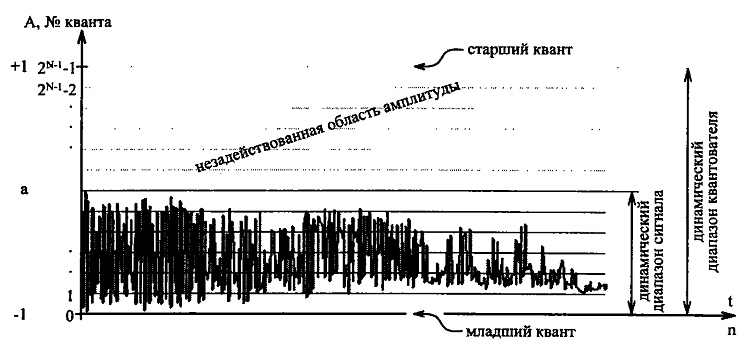
\includegraphics[width=0.75\textwidth]{pic-digital-10}
\caption{Аналогово-цифровое преобразование слабого по уровню аудиосигнала}
\label{pic-digital-10}
\end{figure}

Для уменьшения влияния шума квантования прибегают к использованию приема, называемого \textit{дизерингом}.

\section{Дизеринг и формовка шума}
К \textit{дизерингу} (от англ. "<dithering"> - "<дрожание">) прибегают в тех случаях, когда в результате оцифровки сигнала шум квантования, вместо того чтобы равномерно распределиться по всей полосе полезных частот от 0 до $F_m$, оказывается "<зависимым"> от сигнала, т.е. является своего рода его функцией, в результате чего его спектр оказывается неравномерным, что проявляется на слух в виде возникновения неприятных специфических помех. 

Собственно, так происходит на практике почти всегда, поскольку в практических случаях мы имеем дело с реальными сигналами, параметры которых являются кореллированными. Дизеринг~--- это искусственный прием, который позволяет улучшить субъективное качество звучания
звукового сигнала за счет некоторого умышленного ухудшения его объективных параметров.

\textit{Дизеринг} заключается в намеренном "<подмешивании"> к преобразуемому цифровому сигналу слабого по уровню (с амплитудой в пределах до $2\Delta$) псевдослучайного постороннего сигнала, так называемого дизеринг-шума. Этот, казалось бы, довольно странный прием позволяет придать ошибкам квантования "<более случайный"> характер путем их рассеяния по спектру и тем самым нарушить зависимость
шума квантования от самого преобразуемого сигнала. 

Применение дизеринга приводит фактически к подмене побочных эффектов корреляции шума квантования с преобразуемым сигналом некоторым повышением общей зашумленности сигнала.

Выясняется, что подобное повышение уровня зашумленности сигнала оказывается для слуха более приемлемым, чем побочные эффекты шума квантования.

Применение дизеринга~--- это не единственный метод борьбы с шумом квантования, и в погоне за лучшими результатами квантования были разработаны дополнительные методы, в частности, метод формовки шума.

Идея метода \textit{формовки шума} (noise shaping) следующая~--- преобразовать (точнее~--- перераспределить) шум квантования таким образом, чтобы большая часть его энергии расположилась в наименее заметных на слух частотных областях. 

При правильном применении этого метода можно перераспределить спектр шума квантования таким образом, что общий шум будет менее ощутим на слух, хотя при этом общая энергия шума не изменится.

Применение технологий дизеринга и формовки шума допустимо далеко не всегда. Если аудиоматериал является "<рабочим"> и впоследствии предполагается его дальнейшая обработка и доработка, то использование дизеринга и формовки шума абсолютно недопустимо. Это объясняется следующими причинами. Шум квантования, с таким трудом "<спрятанный"> методом формовки шума под кривой равной громкости, может оказаться оголенным в результате таких операций, как увеличение скорости воспроизведения аудиоматериала, изменение высоты звучания, наложение, микширование и т.д. 

Вместе с тем добавленный дизерингом высокочастотный шум вследствие использования компрессора, сужающего динамический диапазон сигнала, может стать намного более заметным, а также сделать применение алгоритмов сжатия аудиоданных неэффективным. По этим и другим причинам обработку и редактирование аудиоматериалов проводят на гораздо более высокой частоте дискретизации и с более высокой разрядностью, чем предполагаемые значения этих двух параметров для финального аудиоматериала, а дизеринг и формовку шума применяют на самой последней стадии подготовки материала при понижении разрядности и частоты дискретизации.

\section{Джиттер и гранулярный шум}
\subsection{Джиттер}

Управляющая, сопрягающая и преобразующая аппаратура, участвующая в аналогово-цифровом и цифроаналоговом преобразованиях, на практике оказывается далеко не идеальной.

Так, осуществление выборки аналогового сигнала в АЦП может происходить не через абсолютно равные промежутки времени, а с некоторыми случайными отклонениями. Если, например, дискретизация сигнала проводится с номинальной частотой 44,1 кГц, то значения сигнала могут фиксироваться не точно через каждые $1/44100$ c, а перемежаясь то немного раньше, то немного позднее, приводя к регистрации не совсем точного уровня сигнала.

Аналогичная нестабильность может проявляться также на стадии цифроаналогового преобразования в случайных отклонениях длительностей (ширины) прямоугольных импульсов от величины шага дискретизации и в отклонениях крутизны фронтов отдельных импульсов.

Описанный эффект, связанный с несовершенством преобразующей аппаратуры, называется \textit{джиттером} (от англ. "<jitter"> - "<дрожание">) и является исключительно результатом нестабильности в работе АЦП, ЦАП и тактующих схем. На слух джиттер ощущается, как некое "<дрожание"> сигнала на высоких частотах; на низких частотах джиттер выражается в некоторой размытости спектра сигнала. Для
борьбы с джиттером применяют высокостабильные тактовые генераторы.

Следует заметить, что проявление джиттера может наблюдаться не только при аналогово-цифровом и цифроаналоговом преобразованиях сигнала, но также при передаче сигналов по цифровым каналам от одного устройства к другому. В этом случае появление джиттера может быть объяснено несовершенной коммутацией или синхронизацией устройств и устраняется только путем использования специальной сопрягающей аппаратуры, высокоточно корректирующей и регенерирующей цифровой сигнал.

\subsection{Гранулярный шум}
\textit{Гранулярным шумом} (granular noise) называют эффект, проявляющийся при имеющей место нестабильности операции округления в процессе квантования сигнала. 

Если текущая амплитуда сигнала имеет незначительные колебания относительно величины сигнала на границе между двумя соседними уровнями
квантования, то эти даже самые незначительные колебания могут вызывать заметные изменения результатов округления при квантовании значений амплитуды.

Поясним этот эффект на наглядном примере. На рис. \ref{pic-digital-11} показан аудиосигнал, уровень которого располагается приблизительно посередине между двумя ближайшими уровнями квантования $j$ и $j+1$, и амплитуда которого в рассматриваемом временном интервале незначительно колеблется вокруг этого центрального значения.

\begin{figure}[h]
\centering
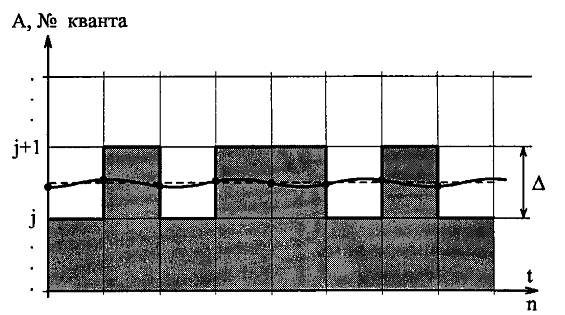
\includegraphics[width=0.75\textwidth]{pic-digital-11}
\caption{Пример возникновения шума квантования}
\label{pic-digital-11}
\end{figure}

Предположим, что используемое в данном случае правило округления при квантовании (способы округления могут быть разными) состоит в округлении измеренного значения амплитуды до ближайшего уровня квантования. Тогда, если амплитуда $А$ сигнала будет находиться ниже значения $A_j+\Delta/2$ ($A_j$~--- уровень сигнала, соответствующий $j$-му кванту), квантователь округлит значение амплитуды до
уровня $j$. 

Если же величина $A$ превысит величину $A_j+\Delta/2$ или станет равной этому значению, то квантователь округлит амплитуду до величины кванта с номером $j+1$.

Результатом квантования рассматриваемого почти постоянного (очень незначительно колеблющегося по уровню) сигнала становится импульсный сигнал, составленный из отсчетов переменной величины; составляющая гранулярного шума в этом импульсном сигнале может оказаться значительной при относительно большом значении $A$. Отсюда можно сделать вывод, что при прочих равных условиях с уменьшением разрядности АЦП уровень гранулярного шума увеличивается.

\section{Неоднородное квантование}
Ранее было отмечено, что между интенсивностью (силой звука) и громкостью звука существует тесная взаимосвязь, в основе которой лежит \textit{закон Вебера-Фехнера}. Этот закон применительно к звуку можно интерпретировать следующим образом: прирост силы слухового ощущения интенсивности (т.е. прирост громкости звука) пропорционален логарифму отношения двух сравниваемых раздражений, т.е. логарифму отношения двух значений интенсивности звука, определяющих этот прирост громкости звука. 

Отсюда следует, что громкость звука, пропорциональная уровню интенсивности звука $L_i$, при прочих равных условиях растет с увеличением интенсивности $I$; при этом любые изменения амплитуды слабого по интенсивности сигнала наша слуховая система различает намного лучше (острее), чем изменения амплитуды в областях высокой интенсивности. Это означает, что погрешность квантования сигнала в областях со слабой амплитудой оказывается намного более заметной на слух, чем погрешность квантования в областях, где сигнал характеризуется высокими значениями интенсивности. Другими словами, в областях, где амплитуда сигнала является значительной, мы можем позволить себе допускать более высокую погрешность квантования, чем в областях со слабой амплитудой. Это обстоятельство и легло в основу метода неоднородного квантования.

Любой способ квантования, предусматривающий использование непостоянного шага $\Delta (\Delta\neq const)$ с наперед заданным разбиением амплитудной шкалы, называется \textit{неоднородным}. 

Здесь мы рассмотрим лишь один из таких способов, называемый логарифмическим квантованием. Логарифмическое квантование предусматривает
разбиение амплитудной шкалы на уровни в соответствии с логарифмическим законом. 

На рис. \ref{pic-digital-12} наглядно продемонстрирована такая амплитудно-временная сетка.

\begin{figure}[h]
\centering
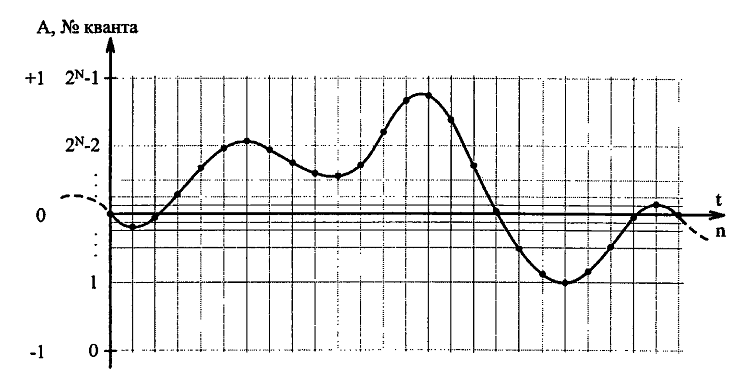
\includegraphics[width=0.75\textwidth]{pic-digital-12}
\caption{Амплитудно-временная сетка при логарифмическом квантовании}
\label{pic-digital-12}
\end{figure}

При использовании логарифмической амплитудной шкалы в области малых значений (низких амплитуд) оказывается большее число уровней квантования, чем в области высоких амплитуд (при этом общее число уровней квантования остается таким же, как и в случае однородного квантования, а именно - $2^N$).

Поэтому при квантовании слабый по амплитуде сигнал округляется на меньшие значения, чем сигнал с более высокой амплитудой, в результате чего обеспечивается эффект субъективного снижения общей погрешности при квантовании звукового сигнала, т.е. погрешность квантования при прочих равных условиях становится менее заметной на слух по сравнению с методом однородного квантования. Здесь следует подчеркнуть, что при логарифмическом квантовании эффект субъективного снижения погрешности квантования получается только за счет использования психоакустических особенностей слуха человека, его способности "<не замечать"> низкий уровень шума на фоне громкого полезного сигнала и выделять тот же уровень шума при малой громкости, т.е. низкой амплитуде полезного сигнала.

Аналогово-цифровое преобразование, основанное на применении метода неоднородного квантования, называется \textit{неоднородной импульсно-кодовой модуляцией}, неоднородной ИКМ (Nonuniform PCM).

\section{Сравнение аналоговой и цифровой форм представления звука}
Когда Эдисон придумал электрическую лампочку, люди горячо спорили о ценности сделанного им изобретения: одни говорили, что идея хороша, но ее практическая реализация слишком накладна, другие вообще смотрели
на изобретение сквозь призму скептицизма, но, конечно, были и те, кто уже тогда предвидел, что изобретение это поистине революционное и что за ним будущее. Так или иначе, но время расставило все по своим местам. Электрическая лампочка пришла на смену газовым фонарям, свечам, коптилкам и всему остальному, светившему "<по старинке">.

Как лампочка Эдисона когда-то осветила людям дорогу в "<электрическое будущее">, так и аналоговые записывающие устройства и аналоговые носители открыли человечеству дорогу в мир звукозаписи. Если до эры звукозаписи большинство людей и подумать не могли о том, что живой звук можно записывать и воспроизводить, то сегодня эта возможность кажется сама собой разумеющейся.

Цифровая форма записи сигналов зародилась одновременно с первыми ЦВМ, в середине 40-х годов XX века. Техника записи, хранения и воспроизведения цифрового звука развивалась очень медленно по сравнению с вычислительной техникой, в частности с ЭВМ. И только в 60-70-х годах, когда появились интегральные микросхемы и ЭВМ на больших интегральных микросхемах, цифровая форма записи звука стала набирать обороты. А с появлением и широким внедрением в быт персональных ЭВМ произошла революция в области записи и цифровой обработки звука.

Цифровой код, описывающий аудиосигнал,~--- это лишь форма, способ представления аналогового аудиосигнала, точно так же как аналоговый аудиосигнал~--- это лишь способ представления реальных звуковых колебаний в воздушной среде. 

Ни аналоговый, ни цифровой сигналы не являются звуком как таковым, кроме самого звука, т.е. колебаний частиц воздушной среды, воздействующих на слуховую систему человека и создающих слуховые ощущения. Именно этот факт и будет основополагающим в наших дальнейших размышлениях.

Вопрос о том, какая форма представления звуковых колебаний лучше, является неоднозначным, поскольку подразумевает сразу три различные трактовки:
\begin{itemize}
\item какая форма представления звуковых колебаний обеспечивает сравнительно более точное приближение к звучанию источника звука;
\item какая форма представления звуковых колебаний обеспечивает наиболее приятное звучание с точки зрения слушателя;
\item какая форма представления звуковых колебаний обеспечивает максимальную компактность, сохранность и предоставляет эффективную возможность преобразования аудиоданных (их монтажа, коррекции и пр.).
\end{itemize}

Звучание на выходе системы тем качественнее, с точки зрения идентичности со звучанием источника звука, чем
меньше стадий обработки и преобразований прошли звуковые колебания на пути от исходного источника звука к слушателю. С этой точки зрения можно считать, что аналоговая аудиоаппаратура выглядит привлекательнее цифровой, поскольку всякая цифровая аппаратура представляет собой как бы надстройку над аналоговой, включая в себя как аналоговый тракт, так и дополнительные цифровые блоки, а значит, звук в цифровой аппаратуре проходит большее число преобразований, чем в аппаратуре аналоговой. Чем больше различных устройств и схем участвует в аудиотракте, тем больше вероятность неверного их сопряжения, состыковки, а значит, тем выше вероятность потерь и искажений сигнала. К этому можно добавить также тот факт, что с точки зрения психоакустики человек заметно более восприимчив к гармоническим (линейным) искажениям, зависящим от самого сигнала, нежели к нелинейным (независящим от сигнала). 
А ведь в основном именно гармонические искажения и сопутствуют цифровым формам представления сигналов, тогда как аналоговая аппаратура привносит в сигнал преимущественно нелинейные искажения (независящие от сигнала), которые менее заметны на слух.

Гармонические (линейные) искажения выражаются в нарушении амплитудных и фазовых соотношений между спектральными компонентами сигнала. Такие искажения воспринимаются на слух, в основном, как искажения тембра.

Негармонические (нелинейные) искажения выражаются в возникновении в спектре сигнала новых паразитных составляющих, отсутствующих в исходном сигнале. Нелинейные искажения являются результатом наличия в аппаратуре нелинейной зависимости выходного сигнала от входного.

Что касается качества звучания, то альтернативный взгляд на это понятие таков: качественным звучанием считается не то звучание, которое максимально приближено к оригинальному, а то, которое положительно воспринимается скажем, среднестатистическим слушателем. Эти два подхода являются принципиально отличными, поскольку первый предполагает объективное сходство воспроизводимого с записи звука с оригинальным, в то время как второй подход является субъективным и такого сходства не предполагает, а предполагает лишь положительное эмоциональное воздействие воспроизводимого звука. Другими словами, не идентичность с исходным сигналом определяет качество выходного
звучания, а тембровая насыщенность, окрас, ясность звучания и т.д.

Существует множество самых различных технологий "<облагораживания"> звучания, которые преобразуют звучание, делая его неидентичным оригинальному, но при этом применение таких технологий "<насыщает"> звук, делает его тембр богаче и красочнее и положительно влияет на эмоции слушателя при восприятии обработанного таким образом звука. Существует также множество технологий, которые призваны "<исправлять"> звучание, искаженное ввиду использования в той или иной степени некачественной или несоответствующей записывающей или обрабатывающей аппаратуры. С точки зрения первого подхода к пониманию качества звучания применение всех таких технологий решительно неуместно, так как они
лишь искажают оригинальное звучание ввиду большого числа стадий обработки. 

При этом описанный второй подход к понимаю качества ни в коем случае не отрицает прямое или косвенное влияние на характер и состав звучания (обработку звука). И даже наоборот, с упором именно на такой подход были созданы технологии, которые путем некоторого уклонения от стремления к идеализированной записи и воспроизведению звука позволили очень заметно экономить объемы данных (речь идет о технологиях кодирования с потерями).

На определенном этапе своего развития аудиоаппаратура, делившаяся когда-то просто на аппаратуру среднего качества и аппаратуру высокого качества, разделилась на два принципиально разных класса: так называемые Hi-Fi и Hi-End. Это
разделение служит ярчайшей иллюстрацией принципиально разных подходов к пониманию понятия "<качество звука">. 

В то время как аппаратура класса Hi-Fi включает самые различные средства обработки звука (фильтры, эквалайзеры, шу
моподавители и т.п.), аппаратура класса Hi-End этого не приемлет~--- здесь нет ничего, что влияет на звучание, кроме ручки громкости. Таким образом, в аппаратуре Hi-Fi к пониманию понятия "<качество звучания"> подходят с точки зрения эмоционального оттенка при восприятии звука, а в аппаратуре класса Hi-End под понятием качества понимают максимальную приближенность звучания к тому живому звучанию, которое было подвержено записи.

Оба описанных подхода к пониманию понятия "<качество звука"> имеют полное право на существование, поскольку оба базируются на вполне логичных вещах. 

Ни один из этих подходов не может быть сочтен эталоном, поскольку оба они относятся к звуку, восприятие и осмысление которого само по себе является делом очень субъективным. На вкус и цвет товарища нет, и каждый должен самостоятельно решить для себя, какой подход ближе лично ему. С уверенностью можно утверждать лишь одно: окажись практическая точность записи, хранения и воспроизведения звука близкой к идеальной, вопрос о вариантах понимания понятия "<качества"> отпал бы сам по себе, поскольку тогда каждый смог бы самостоятельно решать, крутить ему ручки эффект-обработки звука или оставить их в нейтральном положении и слушать лишь абсолютно точную копию настоящего, живого звучания.

На третий из поставленных нами вопросов напрашивается однозначный ответ~--- цифровая форма записи в совокупности с использованием современных цифровых носителей данных является с точки зрения техники записи, хранения и воспроизведения гораздо более удобной и выгодной, чем аналоговая. Даже при допущении стопроцентной сохранности данных на аналоговых носителях возможности аналоговой записывающей аппаратуры по обеспечению высококачественного звучания ограничены~--- они упираются в физические свойства материалов носителей и соображения практической целесообразности использования последних. 

При этом возможности цифровых методов записи и хранения аудиоматериалов почти безграничны. Эта безграничность выражается, например, в том, что в цифровой аппаратуре цифровые данные оказываются абсолютно "<отвязанными"> от носителя и могут свободно переноситься с одного носителя на другой вообще без каких-либо повреждений или искажений, в то время как в аналоговой аппаратуре данные довольно жестко привязаны к носителю (в частности, каждая новая копия фактически никогда не оказывается идентичной другим копиям). 

Практическая безграничность возможностей цифровой аудиоаппаратуры выражается и в том, что возможности улучшения параметров цифровых устройств упираются лишь в совершенство технологий и применяемых алгоритмов, тогда как возможности аналоговой аппаратуры сильно зависят от предела возможностей используемых носителей (эти пределы на практике довольно ограничены).
\end{document}